\documentclass[a4paper,11pt]{article} % screen setting

\usepackage[a4paper]{geometry}
\geometry{verbose,tmargin=1.5cm,bmargin=1.5cm,lmargin=1.5cm,rmargin=1.5cm}

\setlength{\parskip}{\smallskipamount}
\setlength{\parindent}{0pt}

%\usepackage{fontspec}
\usepackage[libertine]{newtxmath}
\usepackage[no-math]{fontspec}
\setmainfont{Linux Libertine O}
\setmonofont{DejaVu Sans Mono}

\usepackage{hyperref}
\usepackage{url}
\usepackage{xcolor}

% DARKMODE
%\pagecolor[rgb]{0,0,0} %black
%\color[rgb]{0.8,0.8,0.8} %grey

\usepackage{amsmath}
\usepackage{amssymb}

\usepackage{graphicx}
\usepackage{float}

\usepackage{minted}

\newminted{dart}{breaklines,fontsize=\footnotesize}
\newminted{bash}{breaklines,fontsize=\footnotesize}
\newminted{text}{breaklines,fontsize=\footnotesize}

\newcommand{\txtinline}[1]{\mintinline[breaklines,fontsize=\footnotesize]{text}{#1}}
\newcommand{\dartinline}[1]{\mintinline[breaklines,fontsize=\footnotesize]{python}{#1}}

\newmintedfile[pythonfile]{python}{breaklines,fontsize=\footnotesize}

\definecolor{mintedbg}{rgb}{0.90,0.90,0.90}
\usepackage{mdframed}
\BeforeBeginEnvironment{minted}{
    \begin{mdframed}[backgroundcolor=mintedbg,%
        topline=false,bottomline=false,%
        leftline=false,rightline=false]
}
\AfterEndEnvironment{minted}{\end{mdframed}}


\usepackage{setspace}

\onehalfspacing

\usepackage{appendix}


\newcommand{\highlighteq}[1]{\colorbox{blue!25}{$\displaystyle#1$}}
\newcommand{\highlight}[1]{\colorbox{red!25}{#1}}


\begin{document}


\title{Pemrograman User Interface dengan Flutter:\\
Pengenalan StatefulWidget}
\author{Fadjar Fathurrahman}
\date{}
\maketitle

\section{Tujuan}

\begin{itemize}
\item Mampu membuat program sederhana berbasis \txtinline{StatefulWidget}
\item Mampu menambahkan aset pada project: image dan audio
\end{itemize}

\section{Desain User Interface}
Pada praktikum ini kita akan membuat suatu user interface yang memiliki
suatu keadaan, yaitu dengan menggunakan \txtinline{StatefulWidget}.
Biasanya \txtinline{StatefulWidget} digunakan pada aplikasi yang memerlukan
interaksi dengan user atau dapat berubah-ubah tampilannya sesuai dengan
keadaan tertentu, misalnya ketika mengupdate data baru dari server.

Berikut ini adalah tampilan aplikasi yang akan kita gunakan.
Aplikasi ini dikembangkan dari aplikasi Counter yang merupakan
contoh default ketika kita membuat project Flutter baru. Perhatikan
bahwa tampilan ini sudah di-resize untuk menghemat ruang pada dokumen ini.
\begin{figure}[h]
{\centering
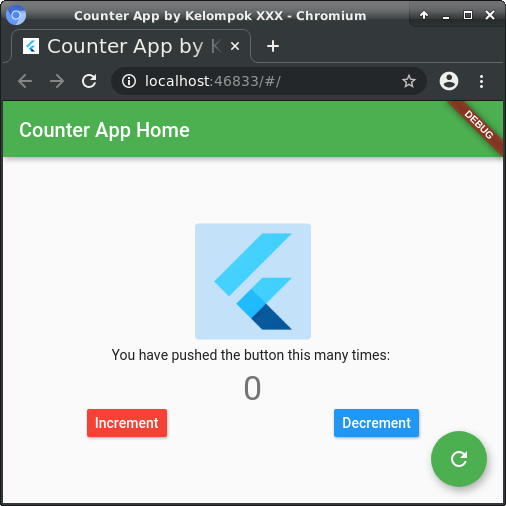
\includegraphics[scale=0.5]{images/counter_app_v2.png}
\par}
\end{figure}

Aplikasi ini terdiri dari beberapa komponen:
\begin{itemize}
\item Logo Flutter (gambar)
\item Teks "You have pushed the button this many times"
\item Teks angka 0
\item Dua button: Increment dan Decrement
\item Floating Button: pada sudut kanan bawah
\end{itemize}

Tiga komponen pertama disusun pada \txtinline{Column} dan
dua button disusun pada suatu \text{Row} (yang akan berada sebagai salah satu
children dari Column). Komponen tersebut kurang lebih akan diimplementasikan
sebagai berikut.
\begin{textcode}
MaterialApp
|- (home): Scaffold
   |- AppBar (appBar of Scaffold)
   |- Center (body of Scaffold)
   |  |- Column
   |     |- Fluttter logo
   |     |- Text
   |     |- Text
   |     |- Row
   |        |- Button Increment
   |        |- Button Decrement
   |- floatingActionButton
\end{textcode}


Sebagai langkah pertama kita akan membuat kode Flutter untuk aplikasi di atas.
Kode yang akan kita buat ini belum memiliki kemampuan untuk berinteraksi dengan
user. Kita akan mengubahnya nanti pada step selanjutnya.

\section{Kode untuk StatelessWidget}
Berikut ini adalah kode Dart untuk desain user interface yang akan digunakan.

\begin{dartcode}
import 'package:flutter/material.dart';

// Starting point dari aplikasi
void main() => runApp(CounterApp());

// Implementasi kelas CounterApp
// Menggunakan MaterialApp, widget home pada MaterialApp akan diimplementasikan
// pada kelas terpisah, yaitu CounterAppHome
class CounterApp extends StatelessWidget {
  @override
  Widget build(BuildContext context) {
    return MaterialApp(
      title: 'Counter App by Kelompok XXX',
      theme: ThemeData(primarySwatch: Colors.green),
      home: CounterAppHome(),
    );
  }
}

// Implementasi kelas CounterAppHome
class CounterAppHome extends StatelessWidget {

  @override
  Widget build(BuildContext context) {
    
    // Logo Flutter, menggunakan Container sehingga dapat dengan mudah
    // diatur padding dan dekorasi yang lain.
    var _flutterLogo = Container(
      margin: EdgeInsets.only(bottom: 5.0),
      padding: EdgeInsets.all(8.0),
      decoration: BoxDecoration(
        color: Colors.blue.withOpacity(0.25),
        borderRadius: BorderRadius.circular(4.0),
      ),
      child: Image.asset(
        'images/flutter_logo_1080.png',
        width: 100,
      ),
    );

    // Button increment, menggunakan RaisedButton yang dibungkus dengan
    // widget Container sehingga lebih mudah untuk diformat.
    // Silakan coba set parameter padding seperti pada _flutterLogo.
    final incrementButton = Container(
      child: RaisedButton(
        child: Text('Increment', style: TextStyle(color: Colors.white)),
        color: Colors.red,
      ),
    );

    // Button decrement
    final decrementButton = Container(
      child: RaisedButton(
        child: Text('Decrement', style: TextStyle(color: Colors.white)),
        color: Colors.blue,
      ),
    );

    // Dua button ini digabung menjadi satu dalam variable _buttons
    var _buttons = <Widget>[incrementButton, decrementButton];

    
    // Gabung seluruh widget diatas pada Scaffold.
    // Seluruh Widget akan diformat dengan rata tengah (Center)
    return Scaffold(
      appBar: AppBar(
        title: Text('Counter App Home'),
      ),
      body: Center(
        child: Column(
          mainAxisAlignment: MainAxisAlignment.center,
          children: <Widget>[
            _flutterLogo,
            Text('You have pushed the button this many times: '),
            Text(
              '0',
              style: Theme.of(context).textTheme.headline4,
            ),
            Row(
              mainAxisAlignment: MainAxisAlignment.spaceAround,
              children: _buttons,
            ), // Row
          ], // <Widget>[],
        ), // Column
      ), // Center
      floatingActionButton: FloatingActionButton(
        tooltip: 'Reset',
        child: new Icon(Icons.refresh),
      ), // FloatingActionButton
    );
  }
}
\end{dartcode}

\section{Menambahkan resource/assets ke dalam project}

Sebelum kita menjalankan aplikasi ini, kita perlu mengedit file
\txtinline{pubspec.yaml}. Hal ini diperlukan karena kita akan menggunakan
file gambar \txtinline{flutter_logo_1080.png}.
Edit file \txtinline{pubspec.yaml} sebagai berikut.
\begin{textcode}
  flutter:
  uses-material-design: true
  assets:
    - images/flutter_logo_1080.png
\end{textcode}
Jika Anda ingin menambahkan gambar lain, silakan edit file ini.

Pada kode yang diberikan, file ini akan ditambahkan ke dalam
direktori bernama \txtinline{images}, yang berada dalam direktori project.
Jika nama project kita adalah \txtinline{counter_app_01}, maka struktur
direktori project akan terlihat sebagai berikut (tidak semua file ditampilkan,
hanya beberapa saja):
\begin{textcode}
  ├── android
  ├── build
  ├── counter_app_01.iml
  ├── images
  │   └── flutter_logo_1080.png
  ├── ios
  ├── lib
  │   └── main.dart
  └── web
\end{textcode}

Jika ada asset lain yang diperlukan, seperti berupa audio atau video, maka
file-file tersebut juga harus ditambahkan pada file
\txtinline{pubspec.yaml}.

File \txtinline{pubspec.yaml} juga perlu diedit jika kita ingin menambahkan
pustaka tambahan atau eksternal selain dari pustaka bawaan dari Flutter.
Kita akan mencobanya pada latihan/tugas.


\section{Pengenalan StatefulWidget}

Berikut ini adalah skenario pada aplikasi yang akan kita buat:
\begin{itemize}
\item ketika user menekan/klik button Increment, maka
tampilan angka akan bertambah sesuai dengan jumlah klik
\item Jika button Decrement ditekan/klik, maka jumlah klik akan berkurang.
\item Jika user floatingActionButton pada kanan bawan diklik maka
jumlah klik akan diatur ulang atau reset menjadi 0.
\end{itemize}
Hal ini mengimplikasikan bahwa aplikasi yang kita buat tidak statik, namun
memiliki suatu keadaan internal atau state (jumlah klik) dan tampilan dari
aplikasi akan bergantung pada nilai dari state (jumlah klik) ini.
Pada Flutter, Widget yang memiliki keadaan atau state internal diimplementasikan
sebagai turunan dari \txtinline{StatefulWidget}.
Kelas yang diturunkan dari \txtinline{StatefulWidget} harus mengimplementasikan
fungsi \txtinline{createState}.

Fungsi \txtinline{creatState} harus mengembalikan suatu objek \txtinline{State},
dalam kasus ini kita membuat kelas \txtinline{_CounterAppHomeState} sebagai
implementasi state dari \txtinline{CounterHomeApp}.
Pada kelas \txtinline{_CounterAppHomeState} inilah kita akan mengimplementasikan
state internal dan user interface dari widget yang akan kita buat.
Pada kelas \txtinline{_CounterAppHomeState} kita harus mendefinisikan
fungsi \txtinline{build} yang sangat mirip dengan kode yang kita gunakan sebelumnya
untuk membangun user interface.

Kode dari \txtinline{CounterAppHome} dan \txtinline{_CounterAppHomeState}
adalah sebagai berikut:
\begin{dartcode}
class CounterAppHome extends StatefulWidget {
  @override
  _CounterAppHomeState createState() => _CounterAppHomeState();
}
  
class _CounterAppHomeState extends State<CounterAppHome> {

  // Variabel atau state dari _CounterAppHomeState
  int _counter = 0;

  // ... kode lainnya

  @override
  Widget build(BuildContext) {

    final incrementButton = ... // teruskan, mirip seperti kode sebelumnya
    // ... kode lainnya
  }
}
\end{dartcode}

Perhatikan bahwa pada kode di atas terdapat satu variabel bernama
\txtinline{_counter} dengan tipe integer yang merepresentasikan jumlah
klik yang dilakukan oleh pengguna. Untuk contoh ini hanya ada
satu variabel state. Pada situasi yang lain mungkin tidak perlu ada
variabel state yang perlu disimpan, dan pada situasi yang lain
bisa jadi ada lebih dari satu variabel keadaan.


\section{Implementasi callback}

Pada kelas \txtinline{_CounterAppHomeState} kita perlu menambahkan dan
dan mengimplementasikan callback atau action handler.
Callback adalah fungsi yang dipanggil ketika suatu action terjadi
pada suatu widget. Action ini berupa properties pada widget yang
biasanya memiliki awalan \txtinline{on}, contohnya:
\begin{itemize}
\item \txtinline{onPressed}
\item \txtinline{onLongPressed}
\end{itemize}
Untuk tipe widget lain, ada banyak action lain yang dapat dimanfaatkan.

Pada contoh ini, kita akan mengimplementasikan callback untuk
\txtinline{onPressed}, yaitu ketika button ditekan biasa.
Kita dapat menginisialisasi \txtinline{incrementButton} sebagai berikut.
\begin{dartcode}
final incrementButton = Container(
  child: RaisedButton(
    child: Text('Increment', style: TextStyle(color: Colors.white)),
    color: Colors.red,
    onPressed: _incrementCounter,
  ),
);
\end{dartcode}
Perhatikan bahwa untuk parameter \txtinline{onPressed} telah diberikan
fungsi \txtinline{_incrementCounter} sebagai callback.
Fungsi \txtinline{_incrementCounter} akan mengubah nilai \txtinline{_counter},
untuk kasus ini menambahkan 1 ke nilai yang ada.
Berikut ini adalah kode untuk melakukan hal tersebut.
\begin{dartcode}
void _incrementCounter() {
  setState( () {
    _counter = _counter + 1;
    print('Increment button is pressed: $_counter');
  } );
}
\end{dartcode}
Perhatikan bahwa fungsi \txtinline{_incrementCounter} memanggil
fungsi \txtinline{setState}
untuk mengimplementasikan aksi (menampilkan pesan ke terminal, bukan ke layar)
dan mengubah variabel \txtinline{_counter}.
Fungsi \txtinline{setState} memerlukan argumen sebuah fungsi, dalam hal ini
kita menggunakan \textit{anonymous function} dengan sintaks:
\begin{dartcode}
() {
  // ... definisi fungsi
}
\end{dartcode}
Sintaks seperti ini sering digunakan sebagai callback.

Selain mengubah nilai \txtinline{_counter}, kita juga perlu mengupdate
tampilan user interface. Dalam hal ini kita akan mengganti angka nol pada
tampilan aplikasi selanjutnya menjadi nilai \txtinline{_counter}.
Perlu dilakukan konversi dari \txtinline{int} menjadi \txtinline{String}
dengan menggunakan metode \txtinline{.toString()}:
\begin{dartcode}
// ... kode lainnya

  Text('You have pushed the button this many times: '),
  Text(
    _counter.toString(), // <-- ganti ini dengan variabel _counter
                         // diubah menjadi string agar dapat ditampilkan
    style: Theme.of(context).textTheme.headline4,
  ),

// ... kode lainnya
\end{dartcode}

\section{Kode lengkap versi 1}
Berikut ini adalah kode lengkap dari aplikasi yang akan kita buat, setelah
dimodifikasi untuk menangani input klik dari user.

\begin{dartcode}
import 'package:flutter/cupertino.dart';
import 'package:flutter/material.dart';
  
void main() => runApp(CounterApp());
  
class CounterApp extends StatelessWidget {
  @override
  Widget build(BuildContext context) {
    return MaterialApp(
      title: 'Counter App by Kelompok XXX',
      theme: ThemeData(primarySwatch: Colors.green),
      home: CounterAppHome(),
    );
  }
}
  
class CounterAppHome extends StatefulWidget {
  @override
  _CounterAppHomeState createState() => _CounterAppHomeState();
}
  
class _CounterAppHomeState extends State<CounterAppHome> {
  
  int _counter = 0;
  
  void _incrementCounter() {
    setState( () {
      _counter = _counter + 1;
      print('Increment button is pressed: $_counter');
    } );
  }
    
  @override
  Widget build(BuildContext context) {
    
    final incrementButton = Container(
      child: RaisedButton(
        child: Text('Increment', style: TextStyle(color: Colors.white)),
        color: Colors.red,
        onPressed: _incrementCounter,
      ),
    );
  
    final decrementButton = Container(
      child: RaisedButton(
        child: Text('Decrement', style: TextStyle(color: Colors.white)),
        color: Colors.blue,
      ),
    );
  
    var _buttons = <Widget>[incrementButton, decrementButton];
    
    var _flutterLogo = Container(
      margin: EdgeInsets.only(bottom: 5.0),
      padding: EdgeInsets.all(8.0),
      decoration: BoxDecoration(
        color: Colors.blue.withOpacity(0.25),
        borderRadius: BorderRadius.circular(4.0),
      ),
      child: Image.asset(
        'images/flutter_logo_1080.png',
        width: 100,
      ),
    );
  
    return Scaffold(
      appBar: AppBar(
        title: Text('Counter App Home'),
      ),
      body: Center(
        child: Column(
          mainAxisAlignment: MainAxisAlignment.center,
          children: <Widget>[
            _flutterLogo,
            Text('You have pushed the button this many times: '),
            Text(
              _counter.toString(),
              style: Theme.of(context).textTheme.headline4,
            ),
            Row(
              mainAxisAlignment: MainAxisAlignment.spaceAround,
              children: _buttons,
            )
          ],
        )
      ),
      floatingActionButton: FloatingActionButton(
        tooltip: 'Reset',
        child: new Icon(Icons.refresh),
      ),
    );
  
  }
}
\end{dartcode}



\section{Latihan 1: implementasi untuk decrement and reset}

Sebagai tugas, coba Anda lengkapi program sebelumnya dengan mengimplementasikan
callback untuk decrement (mengurangi counter dengan 1) dan reset (mengubah counter
menjadi 0).


\section{Latihan 2: Memainkan file audio}

Sebagai latihan lebih lanjut, kita akan membuat aplikasi sebagai berikut.
\begin{figure}[h]
{\centering
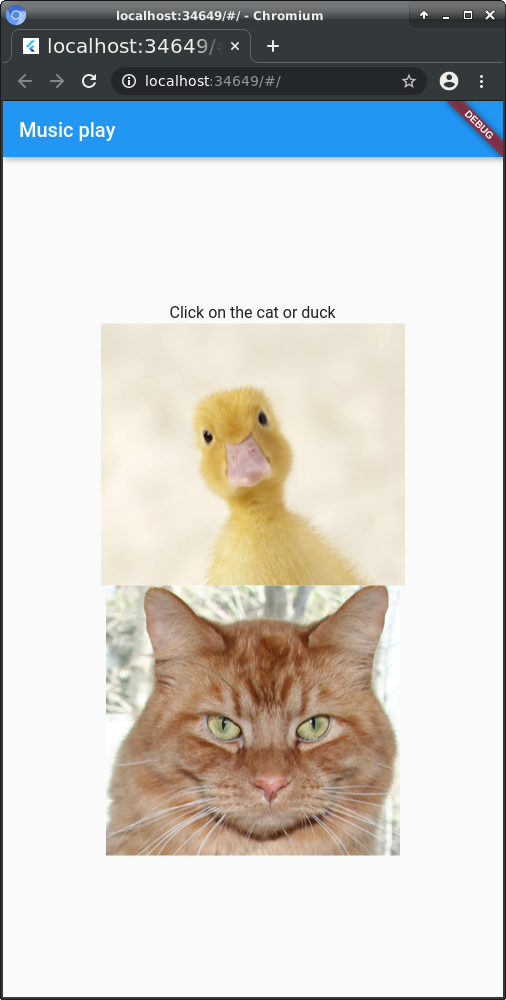
\includegraphics[scale=0.4]{images/DuckCat.png}
\par}
\end{figure}
Aplikasi akan memainkan dua file suara yang berbeda, bergantung dari
gambar mana yang diklik.

Untuk memainkan file audio, kita perlu menggunakan pustaka \txtinline{audioplayers}.
Untuk menggunakan pustaka ini, edit dependensi dapat file \txtinline{pubspec.yaml}
sebagai berikut.
\begin{textcode}
dependencies:
  flutter:
    sdk: flutter
  cupertino_icons: ^1.0.0
  audioplayers: any
\end{textcode}

Kita juga perlu menambahkan beberapa file pada project.
\begin{textcode}
flutter:
  uses-material-design: true
  assets:
    - assets/meow.mp3
    - assets/quack.mp3
    - assets/kitty.png
    - assets/duck.png
\end{textcode}

Anda dapat menggunakan kode berikut ini sebagai referensi.
\begin{dartcode}
import 'package:flutter/material.dart';
import 'package:audioplayers/audioplayers.dart';
  
void main() => runApp(HomePage());
  
class HomePage extends StatefulWidget {
  @override
  _HomePageState createState() => _HomePageState();
}
  
class _HomePageState extends State<HomePage> {
  
  AudioPlayer _audioPlayer = AudioPlayer();
  String _message = 'Click on the cat or duck';
  
  void _playSoundMeow() {
    // ... lengkapi
  }
  
  void _playSoundQuack() {
    // ... lengkapi
  }
  
  @override
  Widget build(BuildContext context) {

    final _buttonCat = FlatButton(
      onPressed: // ... lengkapi,
      padding: EdgeInsets.all(5.0),
      child: Image.asset('assets/kitty.png')
    );

    final _buttonDuck = FlatButton(
      onPressed: // ... lengkapi ,
      padding: EdgeInsets.all(5.0),
      child: Image.asset('assets/duck.png')
    );
  
    final _messageText = Container(
      padding: EdgeInsets.all(2.0),
      child: // ... lengkapi
      )
    );
  
    return MaterialApp(
      home: Scaffold(
        appBar: AppBar(title: Text("Audio play")),
        body: Center(
          child: Column(
            mainAxisAlignment: MainAxisAlignment.center,
            children: <Widget>[
               // ... lengkapi sehingga sesuai gambar
            ]
          ), // Column
        ), // Center
      ) // Scaffold
    ); // MaterialApp
  }
}
\end{dartcode}


Untuk memainkan file audio lokal (pada harddisk komputer/laptop), Anda
dapat menggunakan sintaks sebagai berikut.
\begin{dartcode}
_audioPlayer.play('../assets/meow.mp3', isLocal: true);
\end{dartcode}



\bibliographystyle{unsrt}
\bibliography{BIBLIO}

\end{document}
